\section{Auswertung}

In der folgenden Auswertung werden zuerst die beiden Relaxationszeiten $T\ua{1}$
sowie $T\ua{2}$ bestimmt. Mithilfe von kann dann die Diffusionskonstante $D$ sowie
der Molekülradius bestimmt werden. Der Molekülradius wird am Ende zudem mit
den Radien verglichen, die sich aus dem Molekulargewicht und dem Van-der-Waals-Kovolumen
ergeben.

\subsection{Bestimmung der longitudinalen Relaxationszeit $T\ua{1}$}

Die aufgenommenen Daten für die Bestimmung von $T\ua{1}$ sind Tabelle \ref{tab:T1}
eingetragen sowie in Abbildung \ref{fig:T1} grafisch dargestellt.

\begin{table}
  \centering
  \caption{}
  \label{}
  \begin{tabular}{c | c || c | c}
    \toprule
    $\tau$ in $\si{ms}$ & $U$ in $\si{mV}$ & $\tau$ in $\si{ms}$ & $U$ in $\si{mV}$ \\
    \midrule
    1  & -785 & 100  & -632.5 \\
    2  & -780 & 200  & -565   \\
    3  & -765 & 500  & -395   \\
    5  & -745 & 1000 & -195   \\
    8  & -745 & 1500 &   35   \\
    9  & -735 & 2000 &  118   \\
    13 & -730 & 4000 &  612   \\
    20 & -715 & 7000 &  642.5 \\
    50 & -665 & 9000 &  700   \\
    75 & -647.5 & &           \\
    \bottomrule
  \end{tabular}
\end{table}

\begin{figure}
  \centering
  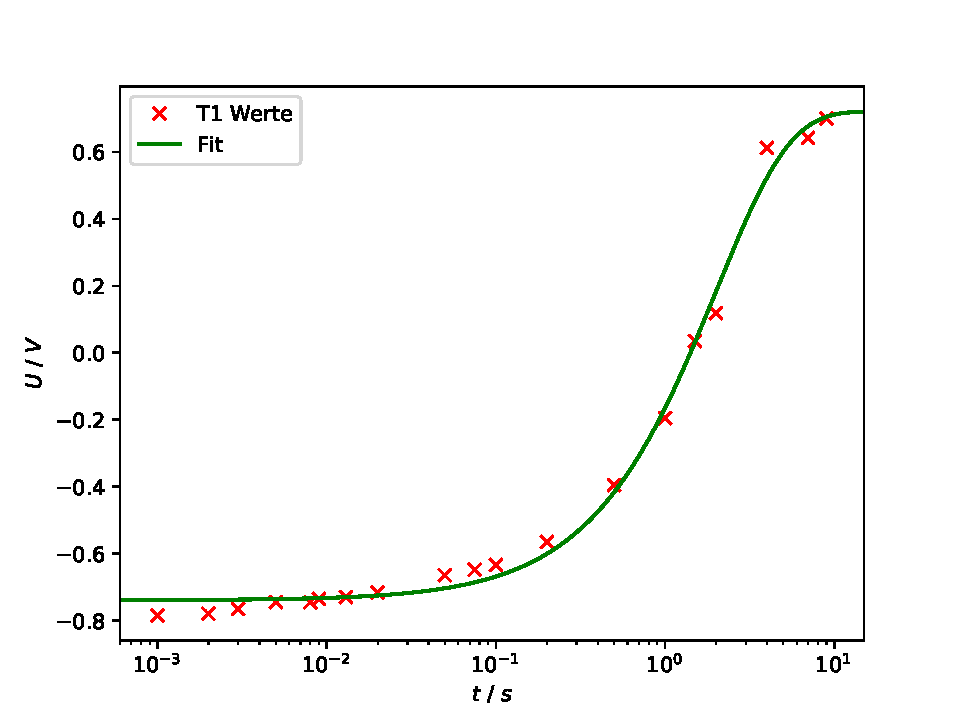
\includegraphics[width=\textwidth]{Plots/T1.pdf}
  \caption{}
  \label{}
\end{figure}
